\section{Appendix}
\label{sec:appendix}

\begin{figure}[H]
	\centering
	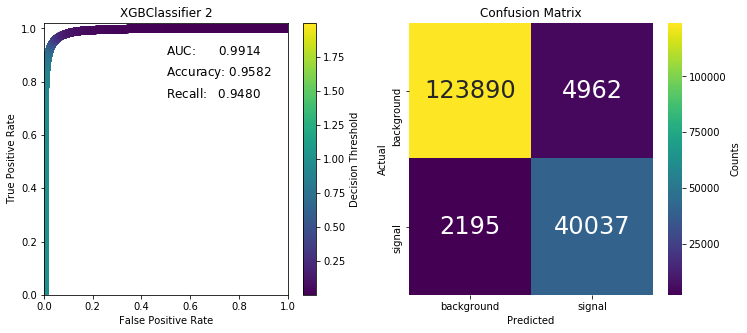
\includegraphics[width=0.8\linewidth]{plots/BDT_2.png}
	\caption{Results and scores of the second BDT.}
	\label{fig:BDT_2}
\end{figure}

\begin{figure}[H]
	\centering
	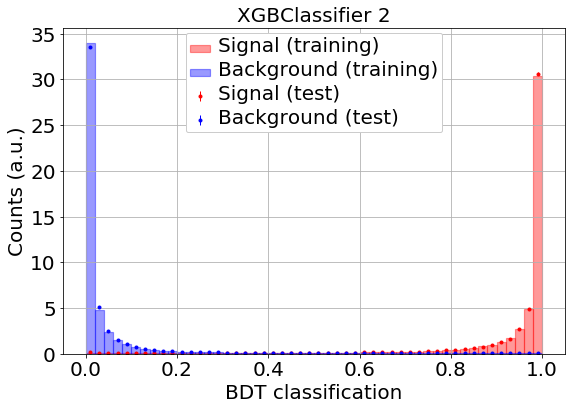
\includegraphics[width=0.5\linewidth]{plots/BDT2_pred.png}
	\caption{Response of the second BDT to training and testing data.}
	\label{fig:BDT_2_pred}
\end{figure}

\begin{figure}[H]
	\centering
	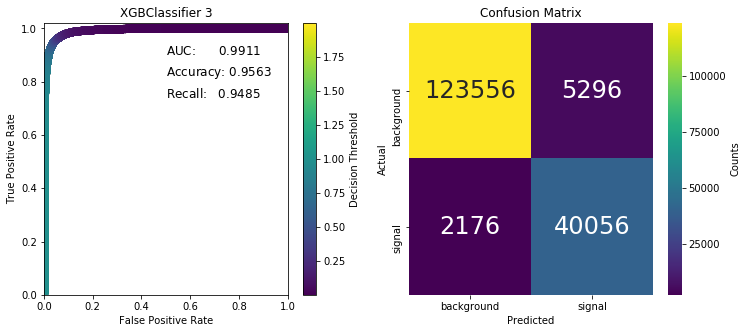
\includegraphics[width=0.8\linewidth]{plots/BDT_3.png}
	\caption{Results and scores of the third BDT.}
	\label{fig:BDT_3}
\end{figure}

\begin{figure}[H]
	\centering
	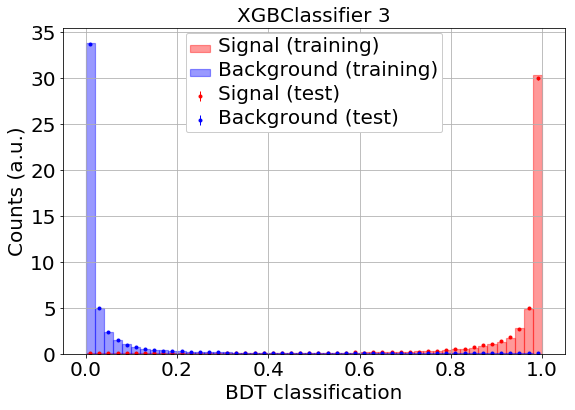
\includegraphics[width=0.5\linewidth]{plots/BDT3_pred.png}
	\caption{Response of the third BDT to training and testing data.}
	\label{fig:BDT_3_pred}
\end{figure}

\begin{figure}[H]
	\centering
	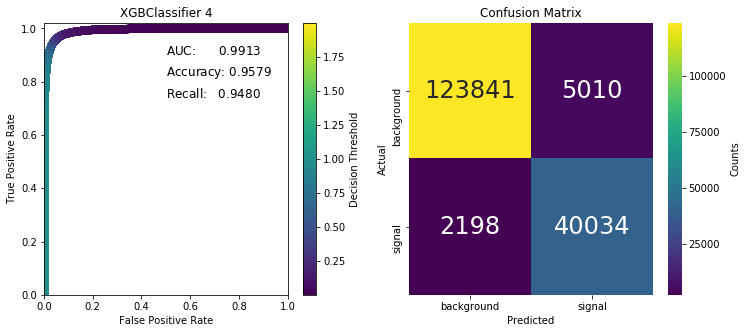
\includegraphics[width=0.8\linewidth]{plots/BDT_4.png}
	\caption{Results and scores of the fourth BDT.}
	\label{fig:BDT_4}
\end{figure}

\begin{figure}[H]
	\centering
	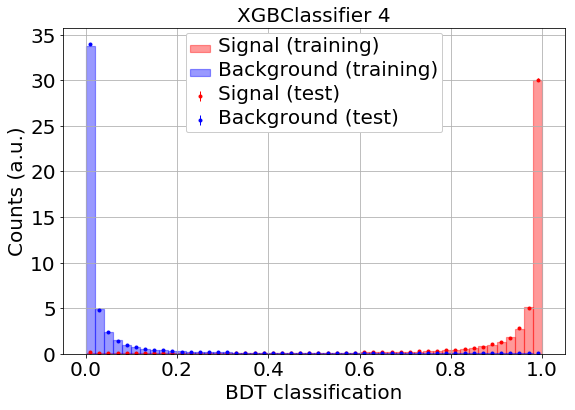
\includegraphics[width=0.5\linewidth]{plots/BDT4_pred.png}
	\caption{Response of the fourth BDT to training and testing data.}
	\label{fig:BDT_4_pred}
\end{figure}

\begin{figure}[H]
	\centering
	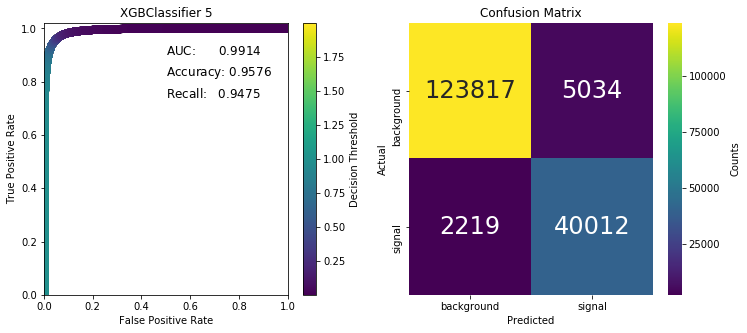
\includegraphics[width=0.8\linewidth]{plots/BDT_5.png}
	\caption{Results and scores of the fifth BDT.}
	\label{fig:BDT_5}
\end{figure}

\begin{figure}[H]
	\centering
	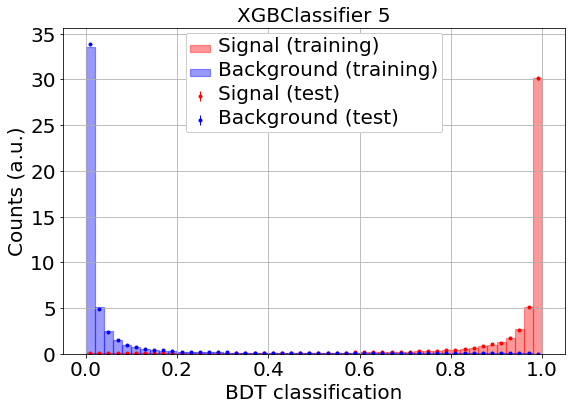
\includegraphics[width=0.5\linewidth]{plots/BDT5_pred.png}
	\caption{Response of the fifth BDT to training and testing data.}
	\label{fig:BDT_5_pred}
\end{figure}